% Chapter Template

\chapter{Methods} % Main chapter title

\label{chap:3:methods} 
% \section{Data Structure}
% \label{sec:methods:data:structure}
% \textcolor{red}{
% \begin{itemize}
%     \item Clinical Data (Including Control) - For both languages, we analyzed the clinical data, consisting of NAP patient sample and a healthy control sample.
%     \item Spoken Semi-Spontaneous Monologue Corpora
%     \item Written Internet Corpora
% \end{itemize}
% }

%-----------------------------------
%	section 1
%-----------------------------------
\section{Data}
\label{sec:methods:data:clinical}

In this chapter, I discuss the data used in the present study (\ref{sec:methods:data:clinical}), as well as the metrics chosen from each of the metric groups (\ref{sec:methods:processing:metrics}) and the ways in which they were computed and analyzed (\ref{sec:methods:stats:clinical})\footnote{The code used for pre-processing the data, calculating the metrics, and post-processing the results is available \href{https://github.com/flying-bear/MA_thesis}{on GitHub} (https://github.com/flying-bear/MA\_thesis, a private repository).}.

\subsection{German}
\label{sec:methods:data:clinical:german}

The German clinical sample consisted of Narrative of Emotions Task \citep{buck2014net} interview recordings from 59 NAP patients\footnote{46 diagnosed with schizophrenia and 13 with schizoaffective disorder.} and 20 controls, characterised in table \ref{tab:data:de:sample}. There was no difference in gender balance, age, or years of education between the groups\footnote{The NAP sample partially coincides with the one described in \citet{just2023validation} for the second time-point. The outpatient data was collected at the Charité hospital in Berlin. The transcription was performed by native German speakers. The data was provided by Dr. Sandra Just.}.

A short version of the narrative emotions task, translated into German, was used. The interview included 3 questions on 4 emotions: sadness, fear, anger, and happiness. The questions were as follows: (1) what does this emotion mean to you? (2) describe a situation where you felt this emotion, and (3) why do you think you felt this emotion in this situation? All interviews were recorded and manually transcribed according to transcription guidelines for establishing the sentence boundaries\footnote{As the LM metrics of the present study operate over sentences, the sentence segmentation decisions can significantly affect the results. To ensure uniformity, the sentence boundaries were determined based on syntax. The sentence was defined as a main clause with all its dependent clauses. Unfinished clauses were delineated as sentences as well. Conjuncted main clauses were separated.}. The interviewer's speech, as well as filled hesitation pauses, were removed from the transcripts. The participant responses were concatenated for each emotion, and the emotions were processed separately and then the values were averaged across emotions. 

% \textcolor{red}{We used the Narrative of Emotions Task (NET, \cite{buck2014net}) to collect speech samples, a short semi-structured interview, originally developed to assess social cognition, at T1. We used a short version of the NET, translated into German, including three questions about four basic emotions: sadness, fear, anger, and happiness: (1) What does this emotion mean to you? (2) Describe a situation where you felt this emotion, and (3) Why do you think you felt this emotion in this situation? All interviews were conducted by trained clinicians, recorded, and manually transcribed, following defined rules for transcription and sentence segmentation. Collecting speech samples from answers to (semi-)structured questions is a frequently used method in NLP studies, increases comparability, and has been shown to outperform analysis of free conversational speech \citep{morgan2021natural}.}

% \textcolor{red}{Uniform sentence annotation guidelines were established for manual coding of sentence boundaries based on syntax, as has been done elsewhere. Clear annotation guidelines for sentence separation are crucial as automated coherence metrics are calculated over sentences and thus, can be influenced by sentence boundary decisions. A sentence was defined as at least containing a subject and verb (e.g., “John eats.”). The main and the corresponding side clauses were grouped together as one sentence (e.g., “John eats when he is hungry.”). Incomplete main clauses were ended on a period (“John eats when. No, I wanted to say something else.”), main clauses connected by conjunction were separated (“John eats when he is hungry. And he laughs when he is happy. And he sleeps when he is tired.”)}

\begin{table}[ht!]
\begin{center}
\begin{tabular}{lllll}
\hline
& \textbf{N} & \textbf{female} & \textbf{age} & \textbf{edu\_years} \\ 
\hline
NAP & 59         & 24              & 39.5 (11.1)  & 14.6 (3.0)               \\
HC  & 20         & 9               & 43.85 (13.3) & 15.5 (2.8)               \\ 
\hline
\end{tabular}
\captionsetup{width=\textwidth}
\caption[German Clinical Dataset]{\label{tab:data:de:sample} Social statistics of the German clinical dataset. Standard deviation is provided in parenthesis for each mean value. ``edu\_years'' indicates years of education.}
\end{center}
\end{table}

For each patient, the SANS, SAPS, and PANSS scores were collected, along with a Verbal IQ score \citep{schmidt1992vocabulary}. The scores for each scale, as well as for PANSS subscales, are characterised in table \ref{tab:data:de:sample:psy}. There was no difference in age, education years, or clinical scale scores between the sexes in the clinical sample. There was also no correlation with years of education or verbal IQ in any of the symptom severity scales. Total SAPS score correlated with PANSS positive subscale, and total SANS score with PANSS negative and general subscales, as well as total PANSS score. As may be expected, PANSS subscales were also intercorrelated, except for PANSS positive, which only correlated with the total score.

Figure \ref{fig:data:de:sample:psy} provides a comparison between the scales for the samples, showing that negative symptoms prevail in the German clinical sample.


\begin{table}[ht]
\resizebox{\textwidth}{!}{%
\begin{tabular}{lllllllllll}
\hline
\textbf{} & \textbf{N} & \textbf{age} & \textbf{edu\_years} & \textbf{Verbal IQ}  & \textbf{SANS} & \textbf{SAPS} & \textbf{PANSS} & \textbf{PANSS\_n} & \textbf{PANSS\_p} & \textbf{PANSS\_o} \\ \hline
range &&&& & 0-120 & 0-170 & 30-210 & 7-49  & 7-49 & 16-112  \\ \hline
all     & 59         & 39.5 (11.1)  & 14.6 (3.0)               & 105.2 (15.7) & 27.7 (20.4)   & 16.8 (16.7)   & 57.3 (16.2)    & 16.9 (6.0)          & 12.7 (5.5)          & 27.8 (7.5)        \\ \hline
male      & 35         & 37.3 (10.1)  & 14.5 (3.1)               & 107.0 (12.7) & 28.6 (21.2)   & 18.6 (16.7)   & 59.2 (17.0)    & 17.1 (6.6)          & 13.4 (5.6)          & 28.6 (7.6)        \\
female    & 24         & 42.7 (11.9)   & 14.7(2.8)                & 102.4 (19.3) & 26.4 (19.4)   & 14.2 (16.7)   & 54.5 (14.8)    & 16.4 (5.2)          & 11.6 (5.2)          & 26.5 (7.3)        \\ \hline
\end{tabular}
}
\captionsetup{width=\textwidth}
\caption[German Clinical Dataset: Psychiatric Scores]{\label{tab:data:de:sample:psy} Clinical statistics of the psychiatric sample in the German clinical dataset. Standard deviation is provided in parenthesis for each mean value. The range is provided for the possible values of the psychiatric scales. \\ ``edu\_years'' indicates years of education.}
\end{table}

\begin{figure}[ht]
\begin{center}
 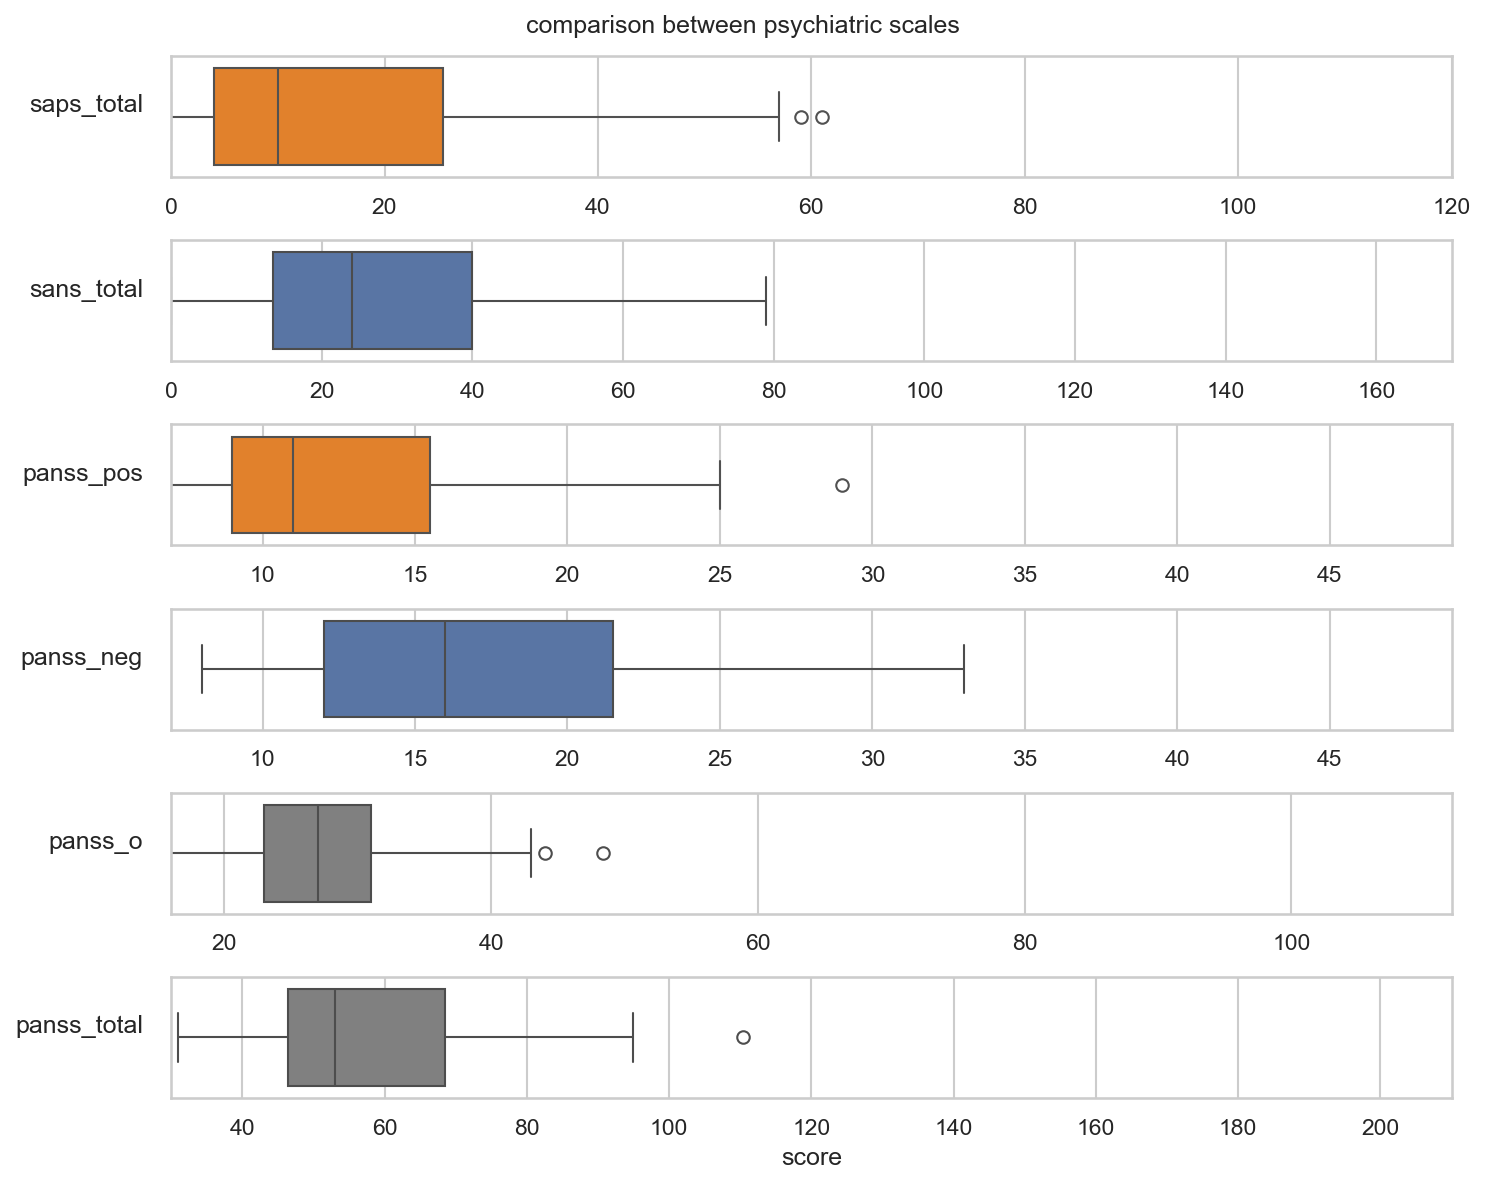
\includegraphics[width=0.6\textwidth]{chapter_3/de_psychiatric.png}  
\captionsetup{width=\textwidth}
\caption[German Clinical Dataset: Psychiatric Scores]{\label{fig:data:de:sample:psy} Clinical statistics of the psychiatric sample in the German clinical dataset. The range corresponds to possible values of the psychiatric scales. Negative symptom scales are shown in blue and positive symptom scales in orange, while grey indicates general symptom scales.}
\end{center}
\end{figure}

\subsection{Russian}
\label{sec:methods:data:clinical:russian}

The Russian clinical sample consisted of monologue speech samples, elicited with 4 tasks, from 31 NAP patients, 18 depressive patients\footnote{The exact diagnosis counts are provided in the appendix \ref{appendix:methods} in table \ref{tab:data:ru:sample:diagnosis}.}, and 30 controls who also underwent a clinical interview process to exclude a possibility of undiagnosed disorders\footnote{The sample partially coincides with the one described in \citet{ryazanskaya2020thesis}. The data was collected jointly by Tatyana Shishkovskaya, Mariya Khudyakova, and me, and transcribed by me. The patient data was collected at the Mental Health Research Center, Moscow.}. 
% , and 102 controls, among whom 30 also underwent a clinical interview process
The sample is characterised in table \ref{tab:data:ru:sample}. There were no differences in age between NAP patients and clinical controls %  (t=2.2, p=0.03)
% ; patients were significantly younger than general controls (t=3.6, p=0.0004)
but there was a significant difference in the years of education between the NAP and control groups (t=3.6, p=0.0006). 
%  and general controls (t=4.7, p=8e-6)
There were no differences between the sexes in any of the samples. It is worth noting that the Russian sample is predominantly female, which is an understudied group when it comes to psychotic disorders, yet this imbalance is a limitation of the present study.

% \begin{table}[h!]
% \begin{center}
% \begin{tabular}{llllll}
% \hline
%     &     & \textbf{N} & \textbf{female} & \textbf{age}  & \textbf{edu\_years} \\ \hline
% NAP &     & 31         & 25              & 27.13 (7.14)  & 13.32 (2.41)        \\
% Dep &     & 18         & 18              & 20.89 (3.71)  & 12.67 (1.94)        \\
% HC  & all & 102 & 75     & 39.75 (19.15) & 15.74 (2.57) \\
%     & psy & 30  & 26     & 25.0 (7.4)    & 15.43 (2.13)        \\ \hline
% \end{tabular}
% \captionsetup{width=\textwidth}
% \caption[Russian Clinical Dataset.]{\label{tab:data:ru:sample} Social statistics of the Russian clinical dataset (only including the participants doing the selected tasks). Standard deviation is provided in parenthesis for each mean value. ``edu\_years'' indicates years of education. ``Dep'' is the sample with predominant depressive symptoms. ``HC psy'' stands for the subset of the healthy patients for which a clinical impression and psychiatric assessment is available.}
% \end{center}
% \end{table}

\begin{table}[ht!]
\begin{center}
\begin{tabular}{lllll}
\hline
    & \textbf{N} & \textbf{female} & \textbf{age}  & \textbf{edu\_years} \\ \hline
NAP & 31         & 25              & 27.13 (7.14)  & 13.32 (2.41)        \\
Dep & 18         & 18              & 20.89 (3.71)  & 12.67 (1.94)        \\
HC  & 30  & 26     & 25.0 (7.4)    & 15.43 (2.13)        \\ \hline
\end{tabular}
\captionsetup{width=\textwidth}
\caption[Russian Clinical Dataset]{\label{tab:data:ru:sample} Social statistics of the Russian clinical dataset (only including the participants doing the selected tasks). Standard deviation is provided in parenthesis for each mean value. ``edu\_years'' indicates years of education. ``Dep'' is the sample with predominant depressive symptoms. ``HC'' stands for the sample of the healthy participants.}
\end{center}
\end{table}

The four tasks used to elicit monologue speech included two picture-elicited tasks (`sportsman' and `adventure'), one instruction task (`chair') and one personal story task (`present')
%\footnote{\textcolor{red}{Other tasks were also available for some of the participants. Only participants who concluded at least one of the four tasks were included in the clinical analysis. \textbf{These texts for the other tasks were used for ...} The description of the entire sample along with the description of other task prompts is provided in \ref{appendix:methods}}}
. The picture description tasks were elicited using two Bidstrup comics, provided in the appendix \ref{appendix:methods}, asking the participant to tell the story depicted in them. The instruction task was elicited using an IKEA chair brochure, asking the participant to instruct a third person, who cannot see the image. Finally, the personal story task was elicited by asking the participant to tell a story about the most memorable present that they had received. As not all participants were able to complete all the tasks, the number of samples available for each task is given in table \ref{tab:data:ru:sample:tasks}. The speech recordings were manually transcribed and separated into sentences according to the same transcription guidelines as the ones used for the German sample. The interviewer's speech, as well as filled hesitation pauses, were removed from the transcripts. 

% \begin{table}[h!]
% \begin{center}
% \begin{tabular}{lllllll}
% \hline
%     &     & N   & adventure & chair & present & sportsman \\ \hline
% NAP &     & 31  & 30        & 17    & 21      & 28        \\
% Dep &     & 18  & 14        & 14    & 13      & 14        \\
% HC  & all & 102 & 55        & 44    & 47      & 54        \\
%     & psy & 30  & 25        & 16    & 19      & 26        \\ \hline
% \end{tabular}
% \captionsetup{width=\textwidth}
% \caption[Russian Clinical Dataset: Task Availability]{\label{tab:data:ru:sample:tasks} Task availability for each selected task in Russian clinical dataset. ``Dep'' is the sample with predominant depressive symptoms. ``HC psy'' stands for the subset of the healthy patients for which a clinical impression and psychiatric assessment is available.}
% \end{center}
% \end{table}

\begin{table}[ht!]
\begin{center}
\begin{tabular}{llllll}
\hline
    & N   & adventure & chair & present & sportsman \\ \hline
NAP & 31  & 30        & 17    & 21      & 28        \\
Dep & 18  & 14        & 14    & 13      & 14        \\
HC  & 30  & 25        & 16    & 19      & 26        \\ \hline
\end{tabular}
\captionsetup{width=\textwidth}
\caption[Russian Clinical Dataset: Task Availability]{\label{tab:data:ru:sample:tasks} Task availability for each selected task in Russian clinical dataset. ``Dep'' is the sample with predominant depressive symptoms. ``HC'' stands for the sample of the healthy participants.}
\end{center}
\end{table}

For each participant, PANSS scores, as well as clinical impressions of thought disorder and depression severity, ranging from 0 to 3, were collected. The scores for each subsample are characterised in table \ref{tab:data:ru:sample:psy}, and figure \ref{fig:data:ru:sample:psy} shows a comparison between the scales in the NAP subsample of the Russian clinical dataset, showing that negative symptoms prevail in this sample. After Bonferroni correction, two of the psychiatric correlated significantly with years of education: PANSS general	(r=-0.41, p\footnote{All p values in this passage are reported as p before correction.}=0.0008) and depression severity (r=-0.33, p=0.003). The psychiatric scores were also intercorrelated. Depression severity correlated with PANSS general (r=0.6, p\textless0.000001) and PANSS total score (r=0.35, p=0.005), as well as thought disorder severity (r=0.33, p=0.003). Thought disorder severity correlated significantly with all other psychiatric scales, most strongly with PANSS positive subscale (r=0.84), total PANSS score (r=0.81), general (r=0.71), and negative (r=0.69) subscales\footnote{All p\textless0.000001.}. All PANSS subscales were significantly intercorrelated with r \textgreater 0.65. 

\begin{table}[ht]
\resizebox{\textwidth}{!}{%
\begin{tabular}{lllllllllllll}
\hline
\textbf{} & \textbf{sex} & \textbf{N} & \textbf{age}                      & \textbf{edu\_years}              & \textbf{Dep} & \textbf{TD} & \textbf{P\_N} & \textbf{PANSS\_TD} & \textbf{PANSS} & \textbf{PANSS\_n} & \textbf{PANSS\_p} & \textbf{PANSS\_o} \\ \hline
range       & & & & & & & &  4-28 & 30-210 & 7-49  & 7-49 & 16-112  \\ \hline
NAP       & all          & 31         & 27.13 (7.14)                      & 13.32 (2.41)                     & 0.58 (0.85)           & 0.84 (0.73)          & 29                        & 10.03 (3.74)       & 69.79 (16.13)  & 22.93 (8.59)        & 15.90 (4.92)        & 30.97 (8.42)      \\ \hline
          & f       & 25         & 27.80 (7.53)                       & 13.56 (2.48)                     & 0.72 (0.89)           & 0.8 (0.76)           & 23                        & 9.43 (3.62)        & 69.13 (15.38)  & 22.52 (7.79)        & 15.3 (4.91)         & 31.3 (9.08)       \\
          & m         & 6          & 24.33 (4.72)                      & 12.33 (1.97)                     & 0.0 (0.0)             & 1.0 (0.63)           & 6                         & 12.33 (3.56)       & 72.33 (20.16)  & 24.5 (11.93)        & 18.17 (4.67)        & 29.67 (5.65)      \\ \hline
Dep       & f       & 18         & 20.89 (3.71)                      & 12.67 (1.94)                     & 0.56 (0.62)           & 0.06 (0.24)          & 13                        & 4.42 (0.9)         & 37.92 (5.89)   & 8.31 (1.97)         & 8.46 (1.94)         & 21.15 (3.58)      \\ \hline
HC & all    & 30 & 25.0 (7.4)   & 15.43 (2.13) & 0.0 (0.0)   & 0.0 (0.0)   & 22   & 4.36 (1.0)   & 30.77 (1.54)  & 7.23 (0.53)  & 7.23 (0.61)  & 16.32 (0.95) \\ \hline
         & f & 26 & 25.42 (7.8)  & 15.42 (1.7)  & 0.0 (0.0)   & 0.0 (0.0)   & 20   & 4.4 (1.05)   & 30.85 (1.6)   & 7.25 (0.55)  & 7.25 (0.64)  & 16.35 (0.99) \\
         & m   & 4  & 22.25 (3.3)  & 15.5 (4.43)  & 0.0 (0.0)   & 0.0 (0.0)   & 2    & 4.0 (0.0)    & 30.0 (0.0)    & 7.0 (0.0)    & 7.0 (0.0)    & 16.0 (0.0)  \\ \hline
\end{tabular}
}
\captionsetup{width=\textwidth}
\caption[Russian Clinical Dataset: Psychiatric Scores]{\label{tab:data:ru:sample:psy} Clinical statistics of the psychiatric sample in the Russian clinical dataset (only including the participants doing the selected tasks). ``HC'' only refers to the subset of the healthy patients. Standard deviation is provided in parenthesis for each mean value. The range is provided for the possible values of the psychiatric scales. \\ ``f'' stands for female; ``m'' for male. ``edu\_years'' indicates years of education; ``P\_N'' indicates the number of participants for whom PANSS scores are available, ``PANSS\_td'' stands for the sum for PANSS questions related to formal thought disorder.}
\end{table}

\begin{figure}[ht!]
\begin{center}
    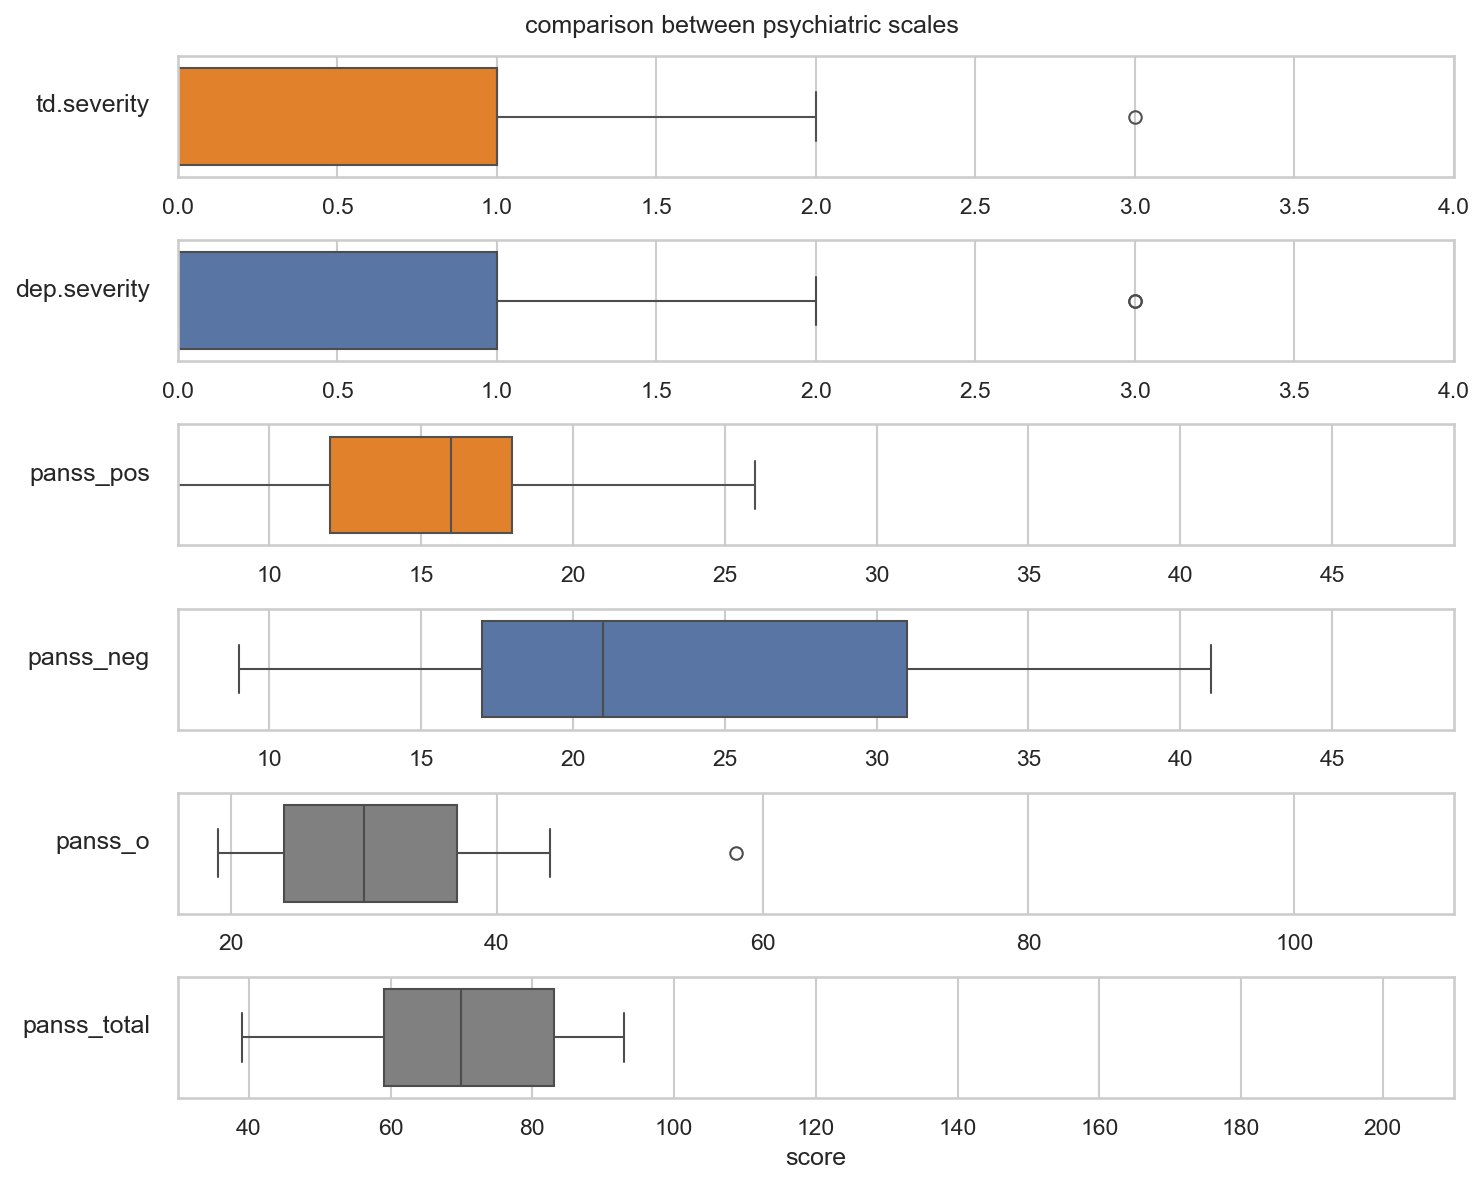
\includegraphics[width=0.6\textwidth]{chapter_3/ru_psychiatric.png}  
\captionsetup{width=\textwidth}
\caption[Russian Clinical Dataset: Psychiatric Scores]{\label{fig:data:ru:sample:psy} Clinical statistics of the psychiatric sample in the NAP subsample of the Russian clinical dataset. The range corresponds to possible values of the psychiatric scales. Negative symptom scales are shown in blue and positive symptom scales in orange, while grey indicates general symptom scales.}
\end{center}
\end{figure}


%-----------------------------------
%	section 2
%-----------------------------------
\section{Data Processing: Metric Pool}
\label{sec:methods:processing:metrics}

Each text in the clinical sample was automatically separated into sentences based on punctuation, tokenised, and lemmatised. The selected metrics, described below, were then computed for each text separately. 

\subsection{Lexical Methods}
As there was little consistency in the use of semantic lexical metrics, only the Lemma-Token Ratio (LTR), Moving Average Lemma-Token Ratio (MALTR), and total word count (n words) were used. LTR was computed as the total number of unique lemmas over the total word count. MALTR was computed as LTR averaged across a moving window of size 10\footnote{The window size was selected to be close to mean sentence length.}, with overlapping windows shifting one word at a time regardless of sentence boundaries. The lemmatization was performed using the SpaCy\footnote{Spacy version 3.7.2.} \texttt{de\_core\_news\_md} and \texttt{ru\_core\_news\_md} models.

\subsection{Syntactic Methods}
The syntactic metrics included sentence parameters such as mean, maximal, and minimal sentence length, along with standard deviation in sentence length, and total sentence count (n sents). Additionally, part-of-speech (POS) rates were used for the POS tested previously: adjectives (ADJ), adverbs (ADV), auxiliary verbs (AUX), coordinating and subordinating conjunctions (CCONJ, SCONJ), determiners (DET), nouns and proper nouns (NOUN, PRPON), pronouns (PRON), particles (PART), and verbs (VERB). The POS tagging was performed using SpaCy models, and the rate was computed as the number of instances of a particular part-of-speech over the total word count.

\subsection{Graph-Based Methods}
The graphs were constructed based on word co-occurrence, as done in \citet{mota2012speech}. The graph construction was performed over lemmas and was performed over a moving window of 100 words\footnote{The moving average approach to graph methods is commonly accepted, and though the window size is not always reported, the 100 words is a common window size. Only few texts were below 100 words in total.}. A pair of lemmas was connected with a directed edge every time they appeared one after the other. The graph metrics included the number of nodes (N)\footnote{The number of nodes corresponds to the unique lemma count calculated over a moving window of size of 100.}, number of edges (E), largest connected component (LCC), largest strongly connected component (LSC), number of parallel edges (PE), number of loops of length one (repeated words), two, and three (L1, L2, L3), average node degree, and standard deviation in the node degree. These characteristics were computed for each window graph and then averaged across the overlapping windows. The characteristics of the graphs were computed using the \texttt{networkx} library.

\subsection{Language Model-Based Methods}
For LM-based methods, three models were compared. First, word2vec, which was loaded via SpaCy interface (obtained from \href{https://fasttext.cc/docs/en/crawl-vectors.html}{fasttext}\footnote{https://fasttext.cc/docs/en/crawl-vectors.html} for \texttt{de} and \texttt{ru})\footnote{Fasttext models at \href{https://fasttext.cc/docs/en/crawl-vectors.html}{fasttext website} are all pretrained on common crawl and Wikipedia dumps.}. Second, built-in SpaCy GloVe models (\texttt{de\_core\_news\_md} and \texttt{ru\_core\_news\_md}). Finally, BERT sentence embeddings (\texttt{bert-base-german-cased} for German and  \texttt{DeepPavlov/rubert-base-cased} for Russian). The two simplest methods of obtaining sentence embeddings from word embeddings were compared for word2vec: simple averaging word vectors (\texttt{w2v\_avg} and \texttt{glove\_avg}) and TF-IDF weighted averaging of word vectors (\texttt{w2v\_tf} and \texttt{glove\_tf}). The word frequencies for TF-IDF were obtained from the \texttt{wordfreq} library\footnote{wordfreq version 3.1.1}. The TF-IDF weighting for word averaging implied giving each word vector a weight of one over the looked-up corpus word frequency, and the `term frequency' was accounted for by the repetition of the word vectors where they were repeated in the sentence. The `CLS' token embedding was used as the BERT sentence vector representation.

Each model sentence vectors were used to compute several coherence scores, namely, local (first order) coherence (\texttt{lcoh}), second order coherence (\texttt{scoh}), global coherence (\texttt{gcoh}) and cumulative global coherence (\texttt{cgcoh}). Local coherence was computed as the mean cosine similarity between the pairs of consecutive sentence vectors. Second-order coherence was computed as the mean cosine similarity between the pairs of sentence vectors with one intervening sentence between them. Global coherence was computed as the mean cosine similarity between each sentence vector and the mean vector of all sentences. Finally, cumulative global coherence was computed as the mean cosine similarity between each sentence vector and the mean vector of all preceding sentences.

A separate representation of the same BERT model was used to estimate pseudo-perplexity (\texttt{pppl}). It was obtained by masking one word at a time and obtaining the pseudo log-likelihood of the word that was masked for each word in a sentence. The pseudo log-likelihoods were then averaged across the sequence and exponentiated to obtain a pseudo-perplexity score\footnote{The calculation was simplified by \href{https://huggingface.co/docs/transformers/perplexity}{passing the true input token ids as labels to the model}, and the loss was simply exponentiated, thus calculating the average masking pseudo log-likelihood for each token in the sentence in one line.}. The metric was averaged across all sentences.

Finally, a separate BERT representation was used to obtain next sentence probability scores for each pair of consecutive sentences (\texttt{sprob}), and the metric was averaged across all sentence pairs. 

\section{Data Analysis}
\label{sec:methods:stats:clinical}

\subsection{Control Variables}
Both samples were analyzed using a two-sided independent t-test for between-group differences in the psycho-social characteristics, as well as for any effects of sex within each group. The psychiatric scales were analyzed for the degree of inter-correlation, as well as for age, education years, and IQ (using Pearson's r). To rule out the effect of age, education years, and IQ, the correlation of the tested metrics with them was computed. Additionally, the correlation of each psycho-social variable with mean sentence length was analyzed to account for results that could stem from the differences in mean sentence length.

\subsection{Target Variables}
Bootstrap was used to evaluate the uncertainty of each metric performance estimate and to account for the effect of the influential points. The data points were drawn with replacements from the sample until the actual sample size was reached; then, the performance was estimated on this sample. For each metric, median value and 25/75 percentiles were used to estimate the metric performance across 1000 iterations.

The performance of each metric was assessed using:
\begin{itemize}
    \item two-sided independent t-test for between-group differences\footnote{The t-test was computed using \texttt{scipy.stats} (version 1.9.1).}. %For the Russian clinical sample, only clinical controls were used in t-test.};
    \item Pearson's r correlation with each psychiatric scale\footnote{The Pearson's r was also computed using \texttt{scipy.stats}.};
    \item ordered categorical regression McFadden’s pseudo r squared for TD and depression severity variables\footnote{The ordered model provided in \texttt{statsmodels} (version 0.13.5) was used.};
    \item Pearson's r correlation with mean sentence length to control for effects explained merely by differences in sentence length.
\end{itemize}

The p-values were not analyzed for the bootstrap, as only the point of the present work is to assess the relative rather than the absolute performance of the metrics\footnote{Due to multiple comparisons, very few if any metrics would remain significant in this benchmark study.}. A metric was considered well-performing if it correlated above 0.3 with any psychiatric scale or had pseudo r squared above 0.09. For the t-test, the metric was well-performing if the 25-75 percentile interval did not cross zero. The metric was considered to be length-dependent if it correlated with mean sentence length above 0.3, yet metrics outperforming the mean sentence length baseline were still considered of interest and analyzed. All were compared for their performance on different psychiatric scales, and for the Russian clinical sample, the metrics were additionally compared for their performance on different tasks. Then the results were compared across languages.


% %----------------------------------------------------------------------------------------
% %	SECTION 2
% %----------------------------------------------------------------------------------------
% \section{Corpus Analysis}
% %-----------------------------------
% %	section 1
% %-----------------------------------
% \section{Spoken Corpus Data}
% \subsection{German}
% \textcolor{red}{DGD}
% \subsection{Russian}
% \textcolor{red}{RusCorpora}


% %-----------------------------------
% %	section 2
% %-----------------------------------
% \section{Web Corpus Data}
% \subsection{German}
% \subsection{Russian}
% \textcolor{red}{Wiki?}


% %-----------------------------------
% %	section 3
% %-----------------------------------
% \section{Corpus Data Processing}
% \label{sec:methods:processing:corpus}
% \textcolor{red}{same metric pool};
% \textcolor{red}{preprocessing, metric application, nan averaging}

% %-----------------------------------
% %	section 4
% %-----------------------------------
% \section{Corpus Data Analysis}
% \label{sec:methods:stats:corpus}

% \textcolor{red}{statistical comparisons?}
